\documentclass[../structure.tex]{subfiles}
%\usepackage{../mypkg}
\begin{document}
\chapter{Method}
\hspace{2em}The main subject of the thesis is demonstrating how the ICP framework can be extended to nonrigid registration, whilst retaining the convergence properties of the original algorithm. The main idea is application of the presented in \cite{Amberg2007}. The resulting optimal step nonrigid ICP framework allows for the use of different regularisations, as long as they have an adjustable stiffness parameter. The registration loops over a series of decreasing stiffness weights and incrementally deforms the template towards the target, recovering the whole range of global and local deformations. To find the optimal deformation for a given stiffness, optimal iterative closest point steps are used. Preliminary correspondences are estimated by a nearest point search. Subsequently, the optimal deformation of the template for these fixed correspondences and the active stiffness is calculated. Afterwards, the process continues with new correspondences found by searching from the displaced template vertices. We present an algorithm using a locally affine regularisation which assigns an affine transformation to each vertex and minimises the difference in the transformation of neighbouring vertices. It is shown that for this regularisation, the optimal deformation for fixed correspondences and fixed stiffness can be determined exactly and efficiently. The method is successful for a wide range of initial conditions, and handles missing data robustly. Furthermore, it is compared qualitatively and quantitatively to other algorithms using synthetic examples and real world data.

\hspace{2em}As it is defined in the introduction that vertex registration is a problem when two or more datsets of points are given and the task is to optimally align them by estimating a best transformation. In our case we use dense registration method to find a mapping from each point in the template onto the target while sparse methods find correspondence only for selected feature points. This is done by deforming the template, localy moving it closer in each iteration to the target in order to wrap them together with respect to stiffnes.

\hspace{2em}ICP moves template $S$ towards target $T$ step by step, in each iteration it minimizes the difference between template $S$ and target $T$ as it shown in figure (\ref{fig:figure1}) to reach the minimal value by solving the main equation (\ref{equ:equation1}) :
\begin{equation}
\label{equ:equation1}
||Ax-b||^2
\end{equation}

\hspace{2em}In equation (\ref{equ:equation1}) $x$ is a list of $X_i$, each $X_i$ is $3\times4$ affine matrix wich use homogeneous coordinates $[x,y,z,1]$ in 3D Euclidean space. By stacking $X_i$ togrther we get $4n\times3$ matrix $x$ as it shown in equation (\ref{equ:equation2}):

\begin{equation}
\label{equ:equation2}
X = [X_1, X_2, ... ,X_n]^T
\end{equation}
If we just solve the equation (\ref{equ:equation1}) by putting $A$ as the template and $b$ as the target, we will get exactly $Ax=b$, which mean the different between them is zero. That lead to deforming $A$ and loss its shape completlly, therefore we need to add stiffnes part to the equation that will prevent this deformation by keeping the vertexes originally close to each others as they are as possible which we will explain later in this chapter.

\begin{figure}[t]
\centering
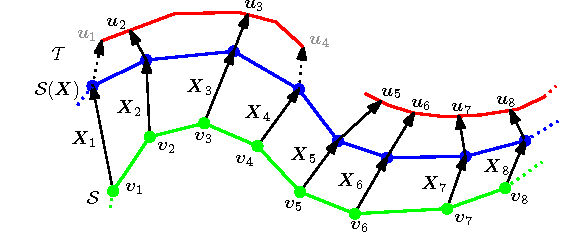
\includegraphics[scale=0.5]{001_conn}
\captionsetup{justification=centering}
\caption{One iteration of ICP, the template $S$ move colser to target $T$ as it became $S(x)$. [source \cite{Amberg2007}]}
\label{fig:figure1}
\end{figure}

\end{document}